\documentclass[10pt]{beamer}

\usetheme{metropolis}
\usepackage{appendixnumberbeamer}

\usepackage{booktabs}
\usepackage[scale=2]{ccicons}

\usepackage{pgfplots}
\usepgfplotslibrary{dateplot}

\usepackage{xspace}
\newcommand{\themename}{\textbf{\textsc{metropolis}}\xspace}

\title{Introduction to GitHub}
%\subtitle{}
\date{\today}
\author{Yann Lamontagne and Sylvain Muise}
\institute{For PedDay2016 at Dawson College}

\begin{document}

\maketitle

\begin{frame}{Table of contents}
  \setbeamertemplate{section in toc}[sections numbered]
  \tableofcontents[hideallsubsections]
\end{frame}

\section{Introduction}

\begin{frame}{What is a version control system?}
A \emph{version control system} is so that your project directory does not look like this\\
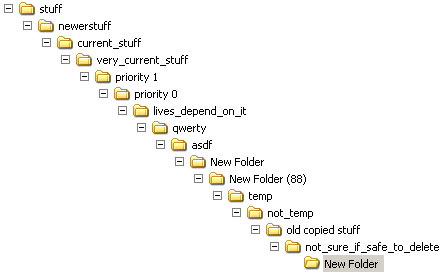
\includegraphics[height=6cm]{images/folders.png}\footnote{from \tt{http://www.dansdata.com/io094.htm}}\\
\end{frame}


\begin{frame}{What is Git?}

\includegraphics[height=1cm]{images/git-logo.png}\\
\tt{git} is a free and open source distributed version control system created Linus Torvalds.\footnote{from \tt{https://git-scm.com/}}
\end{frame}


\begin{frame}{What is GitHub?}

\includegraphics[height=2cm]{images/octocat.png}\footnote{from \tt{https://octodex.github.com/original}}\\
\emph{GitHub} is a web interface to a version control system based on git. 
\begin{itemize}
\item Implements the feature of Git in addition to its own.
\item Has an intuitive app for Windows and Mac.
\end{itemize}

\end{frame}

%\section{Brief Overview of GitHub}

%\begin{frame}
%\end{frame}


\end{document}
